\section{Information Theoretic Security and The One Time Pad}

\subsection{Symmetric Ciphers}

\begin{definition} [Symmetric Cipher] Symmetric Cipher

    Aa cipher defined over $(\mathcal{K}, M, 6) \quad(k, M, c)$ is a pair of "efficient" algs $(\boldsymbol{E}, \boldsymbol{D})$ where 
    $E: \mathcal{K} \times M \rightarrow 6$,  $D: \mathcal{K} \times C \rightarrow \mu$
    s.t. $\forall m \in M, k \in \mathscr{L}: \quad D(k, E(k, m))=m$
    
\end{definition}

\textbf{Notes:}
\begin{itemize} [itemsep=2pt,topsep=0pt,parsep=0pt]
    \item efficient means: can be calculated in a certain polynomial time limit
    \item $E$ is often Randomized
    \item $D$ is always deterministic
\end{itemize}

\subsection{Perfect Security}

\begin{definition} [Shannon Information Theoretic Security] Shannon Information Theoretic Security:

    A cipher $(E, D)$ over $(K, M, C)$ has perfect secrecy if
    $\forall m_{0}, m_{1} \in M \quad\left(\left|m_{0}\right|=\left|m_{1}\right|\right)$ and $\forall c \in C$
    $\operatorname{Pr}\left[E\left(k, m_{0}\right)=c\right]=\operatorname{Pr}\left[E\left(k, m_{1}\right)=c\right]$ where $k \leftarrow^{R} k$
    
\end{definition}

\textbf{Notes: }
\begin{itemize} [itemsep=2pt,topsep=0pt,parsep=0pt]
    \item Given CT, adv. cannot tell if message is $m_0$ or $m_1$
    \item most powerful adv. learns nothing about PT from CT
\end{itemize}


\begin{theorem}
    perfect security $\Rightarrow$ $\mathcal{K} \ge \mathcal{M}$.
\end{theorem}


\subsection{The One-Time Pad: Vernam Cipher}

\begin{definition} [One-Time Pad]

    A one-time pad is a symmetric cipher $\mathcal{E}=(E, D)$, where the keys, messages, and ciphertexts are bit strings of the same length; that is, $\mathcal{E}$ is defined over $(\mathcal{K}, \mathcal{M}, \mathcal{C})$, where
    $$
    \mathcal{K}:=\mathcal{M}:=\mathcal{C}:=\{0,1\}^{L}
    $$
    for some fixed parameter $L$. For a key $k \in\{0,1\}^{L}$ and a message $m \in\{0,1\}^{L}$ the encryption function is defined as follows:
    $$
    E(k, m):=k \oplus m,
    $$
    and for a key $k \in\{0,1\}^{L}$ and ciphertext $c \in\{0,1\}^{L}$, the decryption function is defined as follows:
    $$
    D(k, c):=k \oplus c .
    $$
    
\end{definition}


\begin{theorem} [Inf Secure of OTP] Inf Secure of OTP:

    OTP has perfect security.
    
\end{theorem}


\section{Pseudo Random Generators}


\begin{definition} [Pseudo Random Generators] Pseudo Random Generators:
    $P R G$ is a function $G: \underbrace{\{0,1\}^{s}}_{\text {seed } \atop \text { space }} \rightarrow\{0,1\}^{n} \quad n \gg s$
    (eff. computable by deterministic algorithn )
\end{definition}

\subsection{Security of RPG}

\begin{definition} [negligible and non-negligible] negligible and non-negligible

    $$
    \varepsilon \text { is a function } \varepsilon: \mathbf{Z}^{20} \rightarrow \mathbf{R}^{20} \text { and }
    $$

    $$
    \begin{array}{ll}
    \varepsilon \text { non-neg: } \quad \exists d: \varepsilon(\lambda) \geq 1 / \lambda^{d} \text { inf. often } & (\varepsilon \geq 1 / \text { poly, for many } \lambda) \\
    \varepsilon \text { negligible: } \forall d, \lambda \geq \lambda_{d}: \quad \varepsilon(\lambda) \leq 1 / \lambda^{d} & (\varepsilon \leq 1 / \text { poly, for large } \lambda)
    \end{array}
    $$
        
    
\end{definition}

\begin{method} [Attack Game of Unpred. PRG] Attack Game of Unpred. PRG

    Attack Game 3.2 (Unpredictable $\boldsymbol{P R G}$ ). For a given PRG $G$, defined over $\left(\mathcal{S},\{0,1\}^{L}\right)$, and a given adversary $\mathcal{A}$, the attack game proceeds as follows:
    \begin{enumerate} [itemsep=2pt,topsep=0pt,parsep=0pt]
        \item The adversary sends an index $i$, with $0 \leq i \leq L-1$, to the challenger.
        \item The challenger computes
        $$
        s \stackrel{\mathrm{R}}{\mathcal{S}}, r \leftarrow G(s)
        $$
        \item he adversary outputs $g \in\{0,1\}$.
    \end{enumerate}
    We say that $\mathcal{A}$ wins if $r[i]=g$, and we define $\mathcal{A}$ 's advantage $\operatorname{Predadv}[\mathcal{A}, G]$ to be $\mid \operatorname{Pr}[\mathcal{A}$ wins $]-1 / 2 \mid$.
    
\end{method}

\begin{definition} [Unpredictable PRG] Unpredictable PRG
    A PRG G is unpredictable if the value Predadv[A, G] is negligible for all efficient adversaries A.
\end{definition}

\textbf{Notes: When implementation, never use} \verb!random()! \textbf{for crypto!}

\begin{method} [Attack Game of PRG] Attack Game of PRG
    Attack Game $3.1(P R G)$. For a given PRG $G$, defined over $(\mathcal{S}, \mathcal{R})$, and for a given adversary $\mathcal{A}$, we define two experiments, Experiment 0 and Experiment 1 . For $b=0,1$, we define:
    Experiment $b$ :
    - The challenger computes $r \in \mathcal{R}$ as follows:
    if $b=0: s \longleftarrow \mathcal{R}, r \leftarrow G(s) ;$
    if $b=1: r \longleftarrow{R} \mathcal{R}$.

\end{method}

\begin{definition} [Secure PRG] Secure PRG:

    For $b=0,1$, let $W_{b}$ be the event that $\mathcal{A}$ outputs 1 in Fixperiment $b$. We define $\mathcal{A}$ 's advantage with respect to $G$ as
    $$
    \operatorname{PRGadv}[\mathcal{A}, G]:=\left|\operatorname{Pr}\left[W_{0}\right]-\operatorname{Pr}\left[W_{1}\right]\right|
    $$
    A $P R G G$ is secure if the value $\operatorname{PRGadv}[\mathcal{A}, G]$ is negligible for all efficient adversaries $\mathcal{A}$.
    
\end{definition}

\begin{theorem} [Unpredictable and Secure PRG]

    if $\forall i \in \{0,\cdots,n-1\}$ PRG G is unpredictable at pos. i, then G is a secure PRG.
    
\end{theorem}

\textbf{Notes:} A secure PRG is unpredictable. if next-bit predictors cannot distinguish G from random then no statistical test can


\section{Stream Ciphers: Encrpytion with a PRG}

Idea:  replace "random" key by "pseudorandom" key.

\begin{method} [Stream Cipher] Stream Cipher

    Making OTP practical using a PRG:
    G: $\mathrm{K} \longrightarrow\{0,1\}^{\mathrm{n}}$
    Stream cipher:
    $\mathrm{E}(\mathrm{k}, \mathrm{m})=\mathrm{m} \bigoplus \mathrm{G}(\mathrm{k}) \quad, \quad \mathrm{D}(\mathrm{k}, \mathrm{c})=\mathrm{c} \bigoplus \mathrm{G}(\mathrm{k})$

\end{method}

\section{Attacks on Stream Ciphers and The One Time Pad}

\subsubsection{Two-Time Pad is Insecure}

$$
\begin{aligned}
&c_{1} \leftarrow m_{1} \oplus P R G(k) \\
&c_{2} \leftarrow m_{2} \oplus P R G(k)
\end{aligned}
$$
Eavesdropper does:
$$
\mathrm{C}_{1} \oplus \mathrm{C}_{2} \rightarrow m_{1} \oplus \mathrm{m}_{2}
$$


\textbf{Notes: Never use stream cipher key more than once!}
\begin{itemize} [itemsep=2pt,topsep=0pt,parsep=0pt]
    \item Network traffic: negotiate new key for every session
    \item Disk encryption: typically do not use a stream cipher
\end{itemize}


\subsubsection{One-Time Pad is malleable: not integrity}

Modifications to ciphertext are undetected and  have predictable impact on plaintext

\section{Real-World Stream Ciphers}

\subsection{Old Example: CSS}

The process of CSS is shown in Figure \ref{fig: 02 CSS}.

\begin{figure}[h]
    \centering
    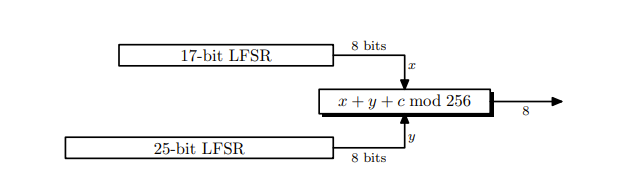
\includegraphics[width=0.8\textwidth]{Stanford_Crypto_1/fig/02_Stream_Cipher/CSS Stream Cipher.png}
    \caption{CSS}
    \label{fig: 02 CSS}
\end{figure}

\subsubsection{Linear feedback shift registers (LFSR)}

The LFSR is a key structure in CSS. The structure of LFSR is shown in Figure \ref{fig: 02 LFSR}.

\begin{figure}[h]
    \centering
    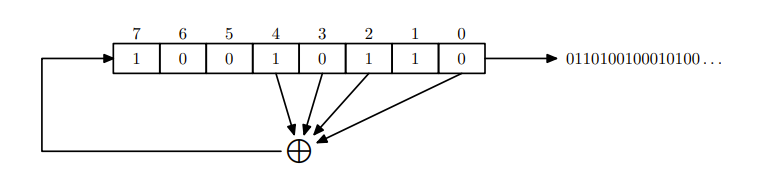
\includegraphics[width=0.8\textwidth]{Stanford_Crypto_1/fig/02_Stream_Cipher/LFSR.png}
    \caption{LFSR}
    \label{fig: 02 LFSR}
\end{figure}


\subsection{Modern Example: eStream: Salsa20}

\subsubsection{eStream Framework}

PRG: $\underbrace{\{0,1\}^{s}}_{\text {seed }} \times R \rightarrow\{0,1\}^{n} \quad n>>s$

\textbf{Nonce}: a non-repeating value for a given key. $R$ is Nonce

$\mathrm{E}(\mathrm{k}, \mathrm{m} ; \mathrm{r})=\mathrm{m} \bigoplus \mathrm{PRG}(\mathrm{k} ; \mathrm{r})$

The pair $(k, r)$ is never used more than once.


\subsubsection{Salsa20}

\begin{equation}
    \begin{aligned}
        &\text { Salsa20: }\{0,1\}^{128 \text { or } 256} \times\{0,1\}^{64} \longrightarrow\{0,1\}^{\mathrm{n}} \quad\left(\max \mathrm{n}=2^{73}\right. \text { bits) } \\
        &\text { Salsa20 }(\mathrm{k} ; \mathrm{r}):=\mathrm{H}(\mathrm{k},(\mathrm{r}, 0))\|\mathrm{H}(\mathrm{k},(\mathrm{r}, 1))\| \ldots
    \end{aligned}
\end{equation}

The structure of Salsa20 is shown in Figure \ref{fig: 02 Salsa20}.

\begin{figure}
    \centering
    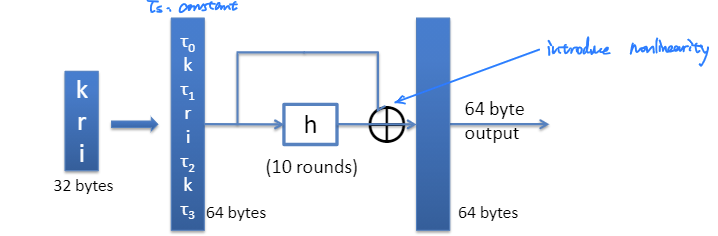
\includegraphics[width=0.6\textwidth]{Stanford_Crypto_1/fig/02_Stream_Cipher/Salsa20.png}
    \caption{Salsa20}
    \label{fig: 02 Salsa20}
\end{figure}

\section{Security Analysis of Stream Ciphers}

\subsection{Semantic Security for One-Time Pad}

\begin{method} [Attack Game for Semantic Security] Attack Game for Semantic Security

    For   $b=0,1$   define experiments EXP(0) and EXP(1) as

    \begin{enumerate} [itemsep=2pt,topsep=0pt,parsep=0pt]
        \item The adversary computes $m0, m1 \in M$, of the same length, and sends them to the challenger.
        \item The challenger computes $k \leftarrow^R K$, $c \leftarrow^R E(k, mb)$, and sends $c$ to the adversary.
        \item The adversary outputs a bit $\hat{b} \in \{0, 1\}$.
    \end{enumerate}


\end{method}



\begin{definition} [Semantic Security] Semantic Security

    For $b=0,1$, let $W_{b}$ be the event that $\mathcal{A}$ outputs 1 in Experiment $b$. We define $\mathcal{A}$ 's semantic security advantage with respect to $\mathcal{E}$ as
    $$
    \operatorname{SSadv}[\mathcal{A}, E]:=\left|\operatorname{Pr}\left[W_{0}\right]-\operatorname{Pr}\left[W_{1}\right]\right|
    $$

    A cipher E is semantically secure if for all efficient adversaries A, the value $SSadv[A, E$] is negligible
    
\end{definition}


\subsection{Stream Ciphers are Semantically Secure}

\begin{theorem} [OPT Sem. Sec.] OPT Sem. Sec.

    OTP is semantically secure
    
\end{theorem}


\section{Summary}

Starting from OTP and the theorem of \textbf{Perfect Security}, we point out the the OTP met the Confidentiality as long as the key length is equal to message length. But it is impossible in practice.

Stream cipher tries to solve this problem by using a key to generate a series of pseudorandom keys. In order to do that, we need to guarantee the process of generate a pseudorandom keys do not harm the security.

So we define what is a secure PRG and relate it with unpredictable. We can also prove that the OTP is Sem. secure with a secure RPG.